\documentclass[]{article}

\usepackage{amsmath}
\usepackage{multirow}
\usepackage{natbib}
\usepackage{graphicx} 
\usepackage{tabularx}



\begin{document}

\title{Quantifying the Temporal Limits of Parameter Identifiability in Damped Harmonic Oscillators}

\author{Denario}
\date{Anthropic, Gemini \& OpenAI servers. Planet Earth.}

\maketitle
\begin{abstract}
The reliability of energy dissipation models for physical systems is fundamentally limited by uncertainty in key parameters like mass and damping. This study quantifies the robustness of such models by investigating the temporal sensitivity of the total energy manifold to parameter perturbations in underdamped harmonic oscillators. Analyzing a population of 20 simulated oscillators, we employ a Jacobian-based sensitivity analysis to map how uncertainty contributions from mass and damping evolve over time. Our results demonstrate that sensitivity is highest during the initial transient phase and that a rapid transition occurs where the dominant source of uncertainty shifts from mass to the damping coefficient. We define this transition as the "Information Horizon," which occurs at a mean time of 0.76 seconds across the population. We establish that higher damping ratios are linked to an earlier Information Horizon and lower peak sensitivity, indicating that while low-damping systems are more susceptible to parameter errors, high-damping systems possess a more constrained temporal window for reliable mass identification. Ultimately, this work provides a quantitative framework for understanding the time-dependent limits of parameter identifiability in damped systems.
\end{abstract}








\section{Introduction}
\label{sec:intro}
The damped harmonic oscillator is a cornerstone model in science and engineering, describing phenomena ranging from the vibrations of civil structures to the dynamics of micro-electromechanical systems. The predictive power of these models is critical for applications such as structural health monitoring, sensor design, and system control. However, the fidelity of any such model is fundamentally limited by the precision of its physical parameters, namely mass, stiffness, and damping. In practice, these parameters are determined through measurement and are thus subject to uncertainty, which can propagate through the model and lead to significant discrepancies between predicted and observed system behavior.

A subtle but critical challenge in modeling these systems is that the influence of parameter uncertainty is not constant over time. As an oscillator evolves and dissipates energy, the sensitivity of its state to different parameters changes. For instance, an error in the system's mass may dominate the energy budget during the initial, high-amplitude oscillations, whereas an error in the damping coefficient may have a more cumulative effect that becomes prominent only at later times. This temporal evolution of parameter influence creates a practical dilemma for system identification: it is unclear which time windows are optimal for reliably estimating a specific parameter. Without a quantitative understanding of these dynamics, experimental design and model validation efforts may be inefficient or misleading.

This paper addresses this challenge by quantifying the temporal limits of parameter identifiability in underdamped harmonic oscillators. We investigate how the sensitivity of the system's mechanical energy, described by the equation $E(t) = \frac{1}{2} m v(t)^2 + \frac{1}{2} k x(t)^2$, responds to perturbations in mass ($m$) and the damping coefficient ($b$). By employing a Jacobian-based sensitivity analysis, we compute the partial derivatives of the energy with respect to each parameter at every time step. This approach allows us to track the time-varying contribution of each parameter to the uncertainty in the system's energy, thereby mapping the evolving landscape of parameter influence directly from the system's dynamics.

Our analysis reveals a distinct and rapid transition in which the dominant source of energy uncertainty shifts from mass to the damping coefficient. We define this critical crossover point as the "Information Horizon," a temporal boundary beyond which the system's dynamics contain more information about dissipative processes than inertial properties. Through the study of a population of simulated oscillators, we demonstrate a systematic relationship between the timing of this horizon and the system's damping ratio. This work establishes a quantitative framework for understanding the time-dependent nature of parameter sensitivity, providing clear insights into the operational limits for robust parameter estimation and model prediction in dissipative systems.

\section{Methods}
\label{sec:methods}
\subsection{Dataset and system model}
Our analysis was performed on a simulated dataset comprising 20 underdamped harmonic oscillators. Each oscillator was defined by a unique set of physical parameters: mass ($m$), stiffness ($k$), and damping coefficient ($b$). The state of each system, described by its time-dependent position $x(t)$ and velocity $v(t)$, was simulated over a 20-second window. The central quantity of interest is the total mechanical energy of the system, $E(t)$, which is governed by the equation:
\begin{equation}
E(t) = \frac{1}{2} m v(t)^2 + \frac{1}{2} k x(t)^2
\label{eq:energy}
\end{equation}
The damping ratio, $\zeta$, was calculated for each oscillator to characterize its damping regime.

\subsection{Jacobian-based sensitivity analysis}
To quantify the temporal sensitivity of the system's energy to its parameters, we employed a Jacobian-based analysis. This method allows for a direct, time-resolved measurement of how perturbations in model parameters influence the energy manifold. For each oscillator at each time step, we computed the Jacobian vector of the energy function with respect to the mass and damping coefficient:
\begin{equation}
\mathbf{J}(t) = \left[ \frac{\partial E}{\partial m}, \frac{\partial E}{\partial b} \right]^T
\label{eq:jacobian}
\end{equation}
The overall sensitivity of the energy manifold at time $t$ was quantified using the Euclidean norm of this vector, defined as the sensitivity index $S(t)$:
\begin{equation}
S(t) = \| \mathbf{J}(t) \|_2
\label{eq:sensitivity_index}
\end{equation}
The individual contributions of mass and damping to the total sensitivity were defined as the partial sensitivities, $S_m(t) = |\frac{\partial E}{\partial m}|$ and $S_b(t) = |\frac{\partial E}{\partial b}|$, respectively. These partial sensitivities allow us to track the evolving dominance of each parameter's influence on the energy uncertainty over time.

\subsection{Quantifying the information horizon}
A primary objective of this study was to identify the temporal point at which the dominant source of energy uncertainty transitions from mass to damping. To this end, we calculated the time-varying sensitivity ratio, $R(t)$, given by:
\begin{equation}
R(t) = \frac{S_b(t)}{S_m(t)}
\label{eq:ratio}
\end{equation}
We define the ``Information Horizon'', $T_H$, as the specific time at which this ratio crosses unity, i.e., when $R(T_H) = 1$. This point marks the transition where the system's energy becomes more sensitive to the damping coefficient than to its mass, representing a fundamental limit for the reliable identification of mass from the energy trajectory.

\subsection{Evaluation metrics and statistical analysis}
To investigate the relationship between system properties and sensitivity dynamics, we performed two key statistical analyses across the population of 20 oscillators. First, we performed a linear regression to model the relationship between the Information Horizon ($T_H$) and the system's damping ratio ($\zeta$). The slope and coefficient of determination ($R^2$) were calculated to quantify the strength and direction of this trend. Second, we examined the link between the peak sensitivity observed during the transient phase, $S_{max} = \max(S(t))$, and the damping ratio. The Pearson correlation coefficient ($\rho$) was computed to assess the association between these two variables.

\section{Results}
\label{sec:results}
The sensitivity of the total mechanical energy to perturbations in mass and damping was evaluated over time for the population of 20 simulated oscillators. Our analysis reveals a distinct temporal evolution in parameter influence, culminating in a rapid transition that defines the limits of parameter identifiability.

\subsection{Temporal evolution of energy sensitivity}
The overall sensitivity of the energy manifold to parameter perturbations was quantified using the sensitivity index $S(t)$, as defined in Equation \ref{eq:sensitivity_index}. Figure \ref{fig:sensitivity_heatmap} displays a heatmap of $S(t)$ for all 20 oscillators over the 20-second simulation period. The results consistently show that sensitivity is highest during the initial transient phase of the oscillation, typically within the first two seconds. Following this peak, the sensitivity index decays exponentially, mirroring the dissipation of mechanical energy in the system. This indicates that the energy manifold is most susceptible to parameter uncertainties at the beginning of the system's evolution, when kinetic and potential energies are at their maximum.

\begin{figure}[h!]
    \centering
    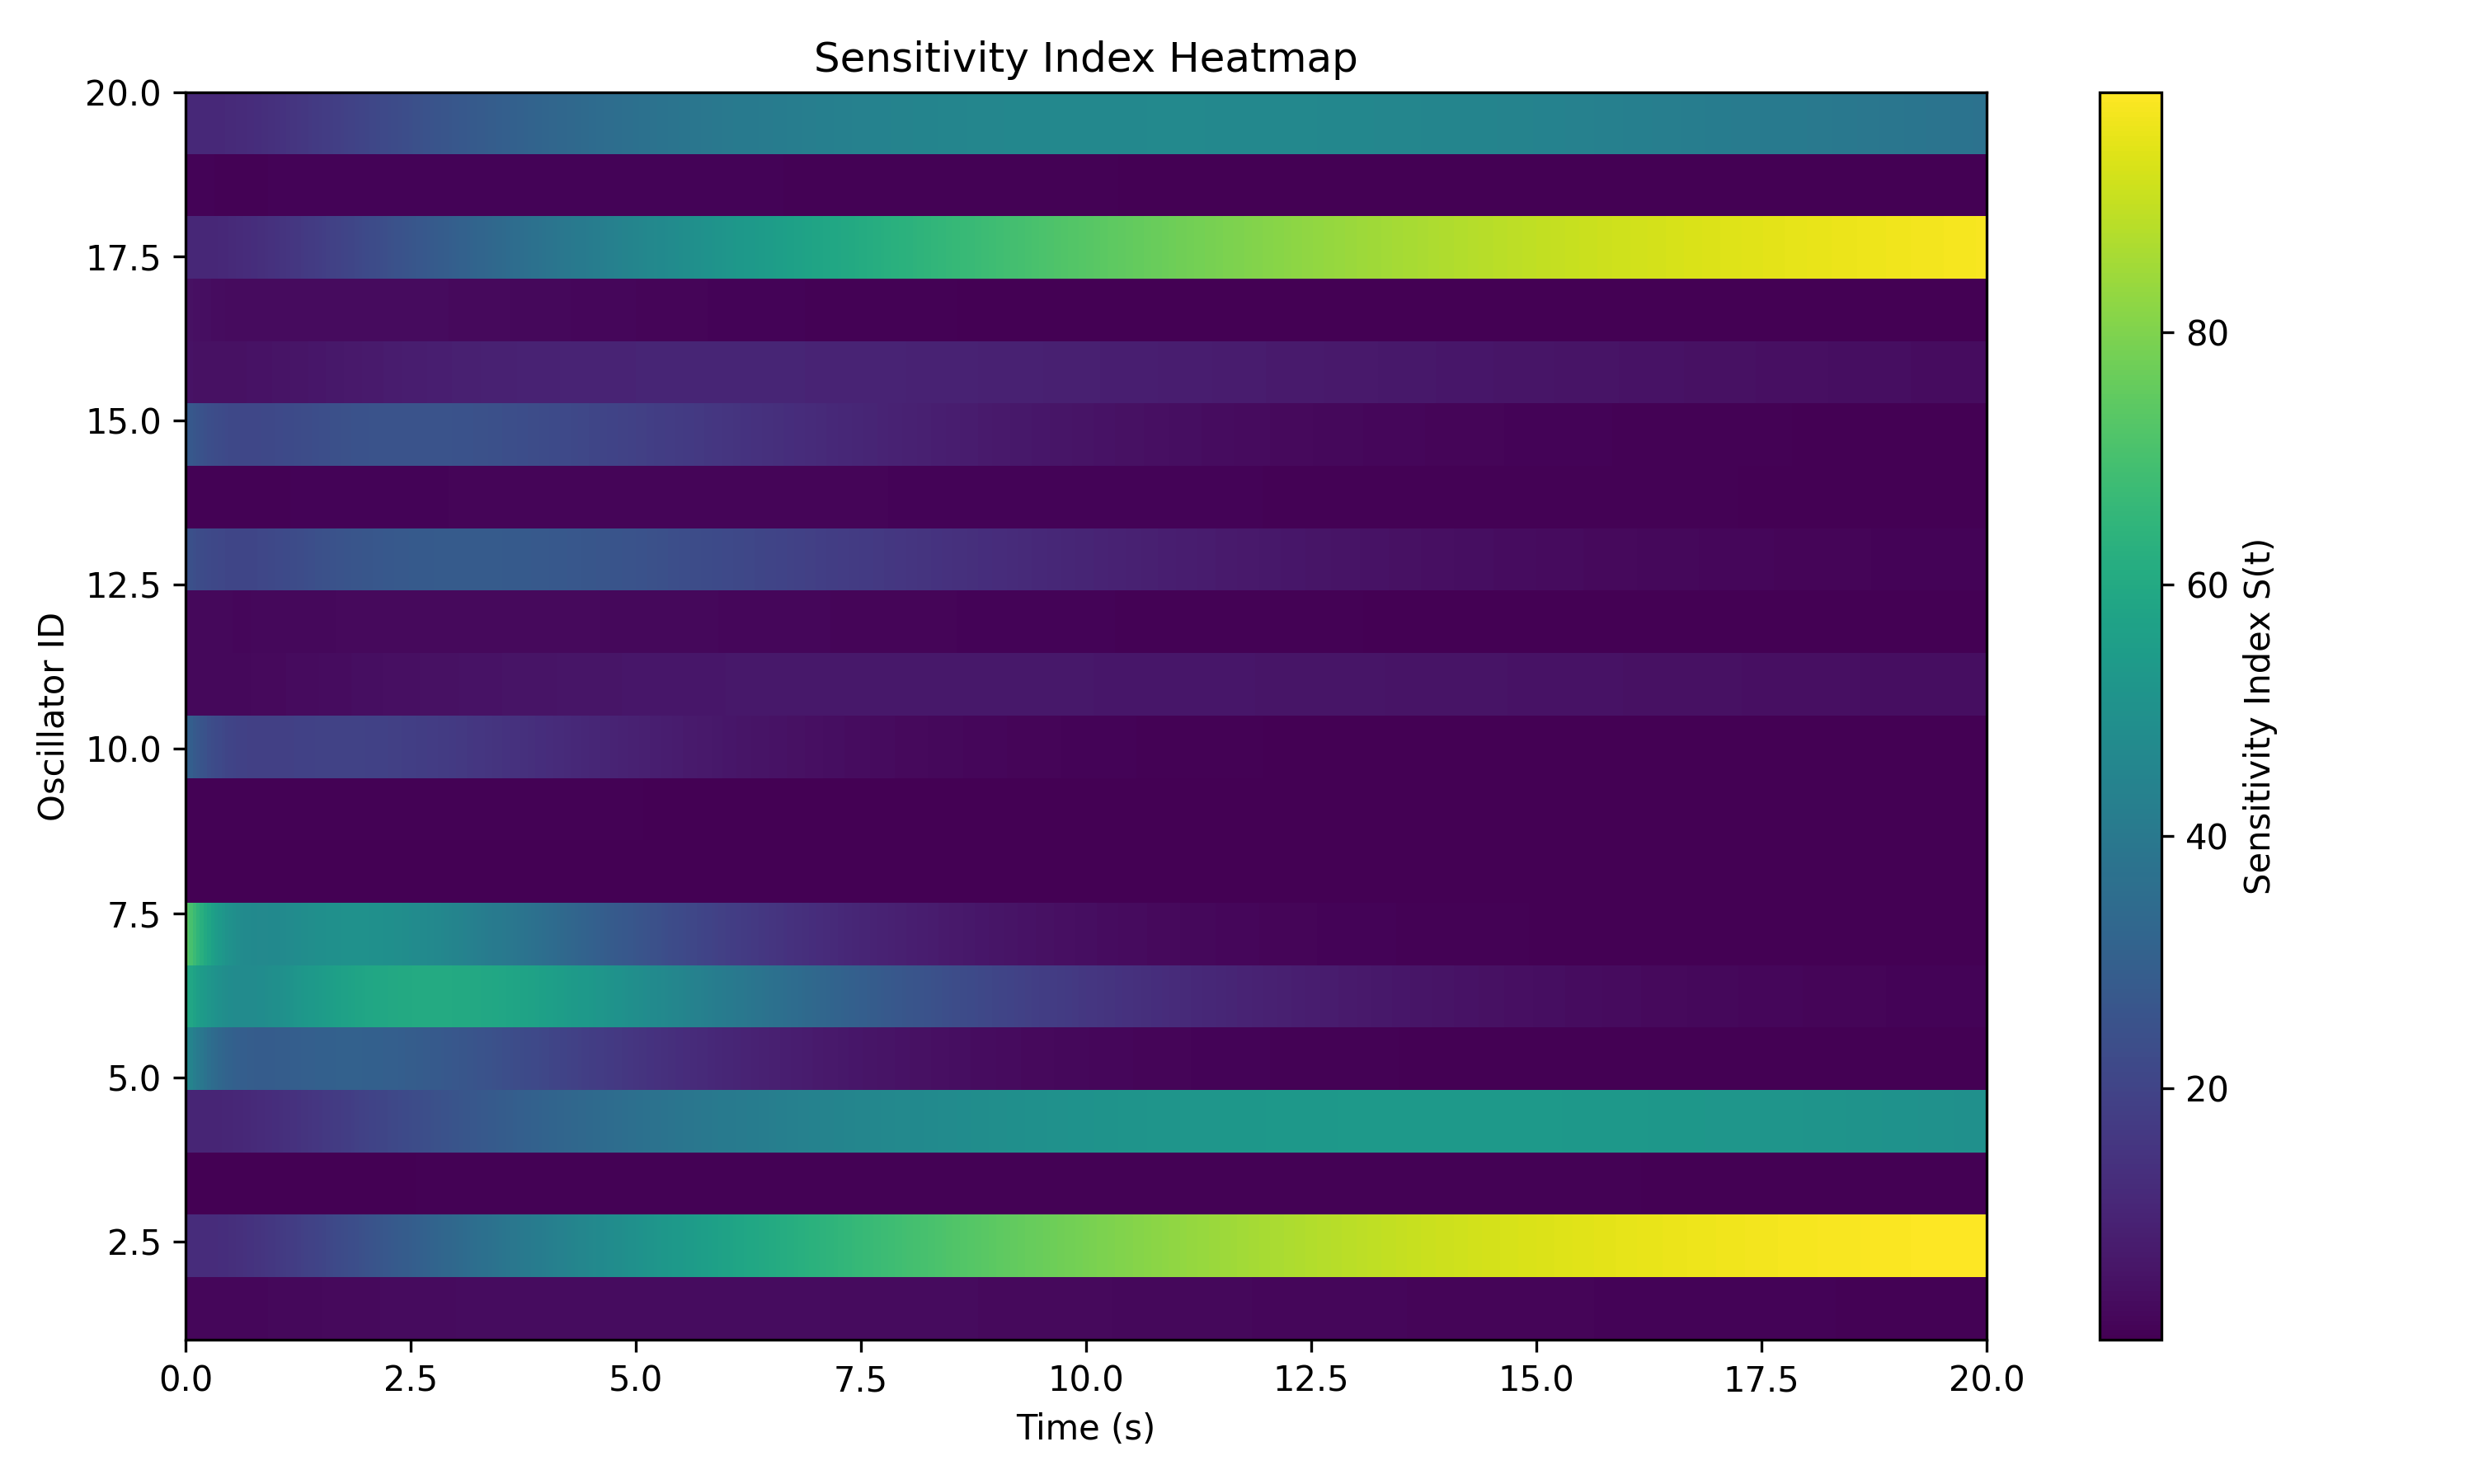
\includegraphics[width=\columnwidth]{../input_files/plots/step_2_sensitivity_heatmap_1739965000.png}
    \caption{Temporal evolution of the sensitivity index, S(t), for 20 distinct underdamped oscillators over a 20-second interval. The color intensity corresponds to the sensitivity of the total energy model to perturbations in mass and damping parameters. The plot reveals that sensitivity is highest during the initial transient phase (t < 2s) and subsequently decays, demonstrating that the energy manifold is most susceptible to parameter estimation errors shortly after the initial state.}
    \label{fig:sensitivity_heatmap}
\end{figure}

\subsection{The information horizon and the shift in parameter dominance}
To understand the sources of this time-varying sensitivity, we decomposed the sensitivity index into its partial contributions from mass, $S_m(t)$, and the damping coefficient, $S_b(t)$. The temporal evolution of these partial sensitivities, shown in Figure \ref{fig:sensitivity_evolution}, reveals a clear and consistent pattern across all simulated oscillators. The sensitivity to mass, $S_m(t)$, dominates during the initial phase, driven by the large contribution of the kinetic energy term ($\frac{1}{2}mv^2$) to the total energy. As the system evolves and energy dissipates, the sensitivity to the damping coefficient, $S_b(t)$, which governs the rate of energy decay, grows in relative importance and eventually surpasses the sensitivity to mass.

This transition marks a fundamental shift in the information content of the system's energy trajectory. We define the point of this transition as the ``Information Horizon'', $T_H$, which occurs when the sensitivity ratio $R(t) = S_b(t)/S_m(t)$ crosses unity (see Equation \ref{eq:ratio}). Beyond this horizon, the system's energy provides more information about dissipative processes than about its inertial properties. Across the population of oscillators, the Information Horizon occurred at a mean time of $0.76$ seconds, with all instances occurring between 0.60 s and 0.92 s. This demonstrates that the shift in parameter dominance is a rapid phenomenon that happens early in the system's evolution.

\begin{figure}[h!]
    \centering
    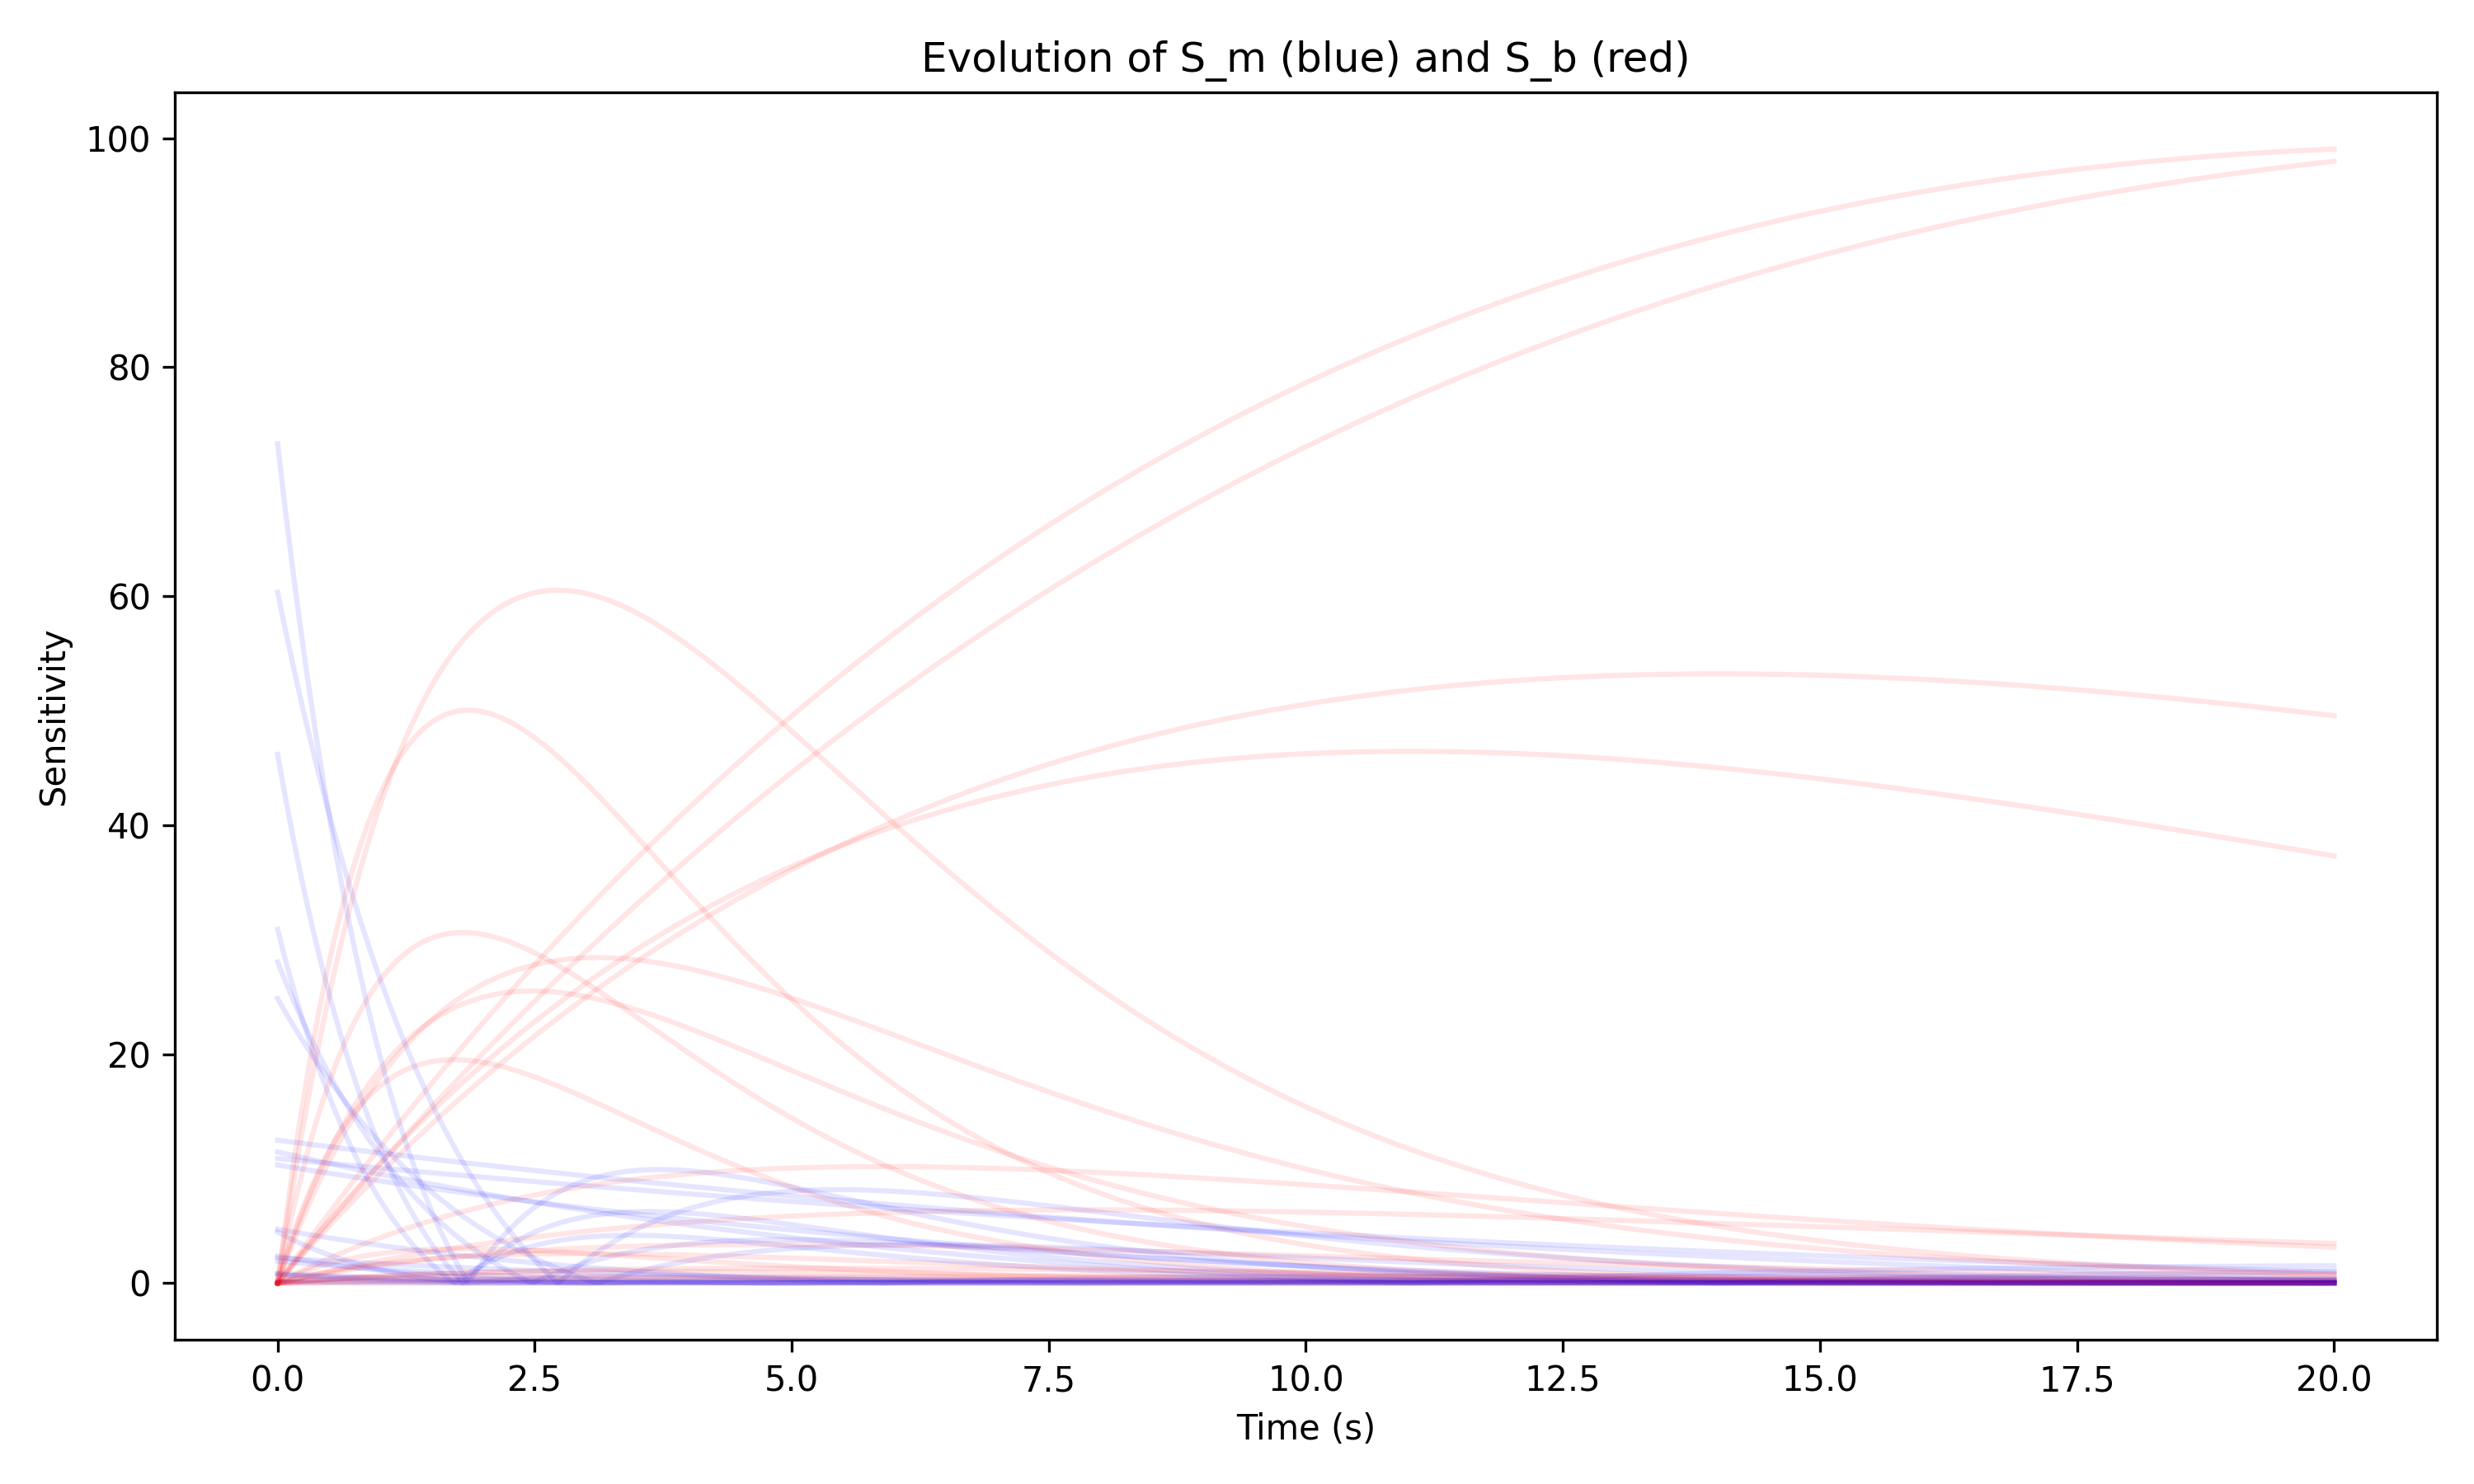
\includegraphics[width=\columnwidth]{../input_files/plots/step_2_sensitivity_evolution_1739965000.png}
    \caption{Temporal evolution of the partial sensitivities of total energy with respect to mass ($S_m$, blue) and the damping coefficient ($S_b$, red) for 20 distinct underdamped oscillators. The plot illustrates a rapid regime shift where the initial dominance of mass-related sensitivity ($S_m$) transitions to a dominance by damping-related sensitivity ($S_b$). This crossover, defining the Information Horizon ($T_H$), consistently occurs early in the transient phase (t < 1s), indicating that the energy model's uncertainty is primarily governed by the damping parameter for the majority of the system's evolution.}
    \label{fig:sensitivity_evolution}
\end{figure}

\subsection{Relationship between damping ratio and sensitivity dynamics}
To investigate the factors governing these sensitivity dynamics, we analyzed the relationship between the system's damping ratio, $\zeta$, and two key metrics: the timing of the Information Horizon, $T_H$, and the peak sensitivity observed during the transient phase, $S_{max}$. The results of this statistical analysis are summarized in Table \ref{tab:stats_summary}.

\begin{table}[h!]
\centering
\caption{Statistical summary of the relationship between the damping ratio ($\zeta$) and key sensitivity metrics across the population of 20 oscillators.}
\label{tab:stats_summary}
\begin{tabular}{lc}
\hline
\hline
Metric & Value \\
\hline
Mean Information Horizon ($T_H$) & 0.76 s \\
Slope ($T_H$ vs. $\zeta$) & -0.8347 \\
$R^2$ (Regression of $T_H$ on $\zeta$) & 0.3326 \\
Correlation ($\rho$) of $S_{max}$ vs. $\zeta$ & -0.5221 \\
\hline
\end{tabular}
\end{table}

A linear regression analysis reveals a negative relationship between the Information Horizon and the damping ratio, with a slope of -0.8347. This indicates that systems with higher damping ratios experience an earlier transition to damping-dominated sensitivity. In other words, a higher $\zeta$ shortens the temporal window in which mass can be reliably identified from the energy trajectory. The coefficient of determination ($R^2 = 0.3326$) suggests that the damping ratio explains a moderate portion of the variance in the timing of $T_H$.

Furthermore, we found a moderate negative Pearson correlation ($\rho = -0.5221$) between the peak sensitivity, $S_{max}$, and the damping ratio. This implies that oscillators with lower damping are more sensitive to parameter perturbations during their initial, high-energy phase. While these low-damping systems offer a longer window for mass identification before the Information Horizon, their energy manifolds are inherently more susceptible to errors in parameter estimation during this critical period. Conversely, high-damping systems are less sensitive overall but offer a more constrained window for identifying inertial properties.

\section{Conclusions}
\label{sec:conclusions}


This paper addressed the challenge of time-dependent parameter identifiability in damped harmonic oscillators, where the influence of parameters such as mass and damping on system dynamics evolves over time. Our objective was to quantify the temporal limits within which these parameters can be reliably estimated from the system's energy trajectory. To achieve this, we employed a Jacobian-based sensitivity analysis on a simulated dataset of 20 underdamped harmonic oscillators. We computed the partial derivatives of the total mechanical energy with respect to mass and the damping coefficient at each time step, allowing us to track the evolving contribution of each parameter to the model's uncertainty.

Our results demonstrate that the sensitivity of the system's energy to its parameters is highest during the initial transient phase and decays exponentially thereafter. We identified a distinct and rapid transition in which the dominant source of energy uncertainty shifts from the mass to the damping coefficient. We defined this crossover point as the ``Information Horizon'', which occurred at a mean time of 0.76 seconds across the population. This finding establishes a clear temporal boundary beyond which the system's energy contains more information about dissipative processes than its inertial properties.

From these results, we have learned that a fundamental relationship exists between a system's damping characteristics and its parameter identifiability. Specifically, we found that higher damping ratios lead to an earlier Information Horizon and lower peak sensitivity. This reveals a critical trade-off: systems with low damping provide a longer temporal window for reliable mass identification but are more susceptible to parameter errors during this period. Conversely, highly damped systems are less sensitive to parameter perturbations but offer a much more constrained time frame for estimating mass. Ultimately, this work provides a quantitative framework for understanding the operational limits of model-based analysis in dissipative systems and offers a practical guideline for designing more effective system identification experiments.


\bibliography{bibliography}{}
\bibliographystyle{unsrt}

\end{document}
